% !TeX root = RJwrapper.tex
\title{A package for Cleaning and Analyzing Coursera OnDemand Data}
\author{by Aboozar Hadavand, Jeffrey Leek}

\maketitle

\abstract{%
An abstract of less than 150 words.
}

\subsection{Introduction}\label{introduction}

It is hard to pin down the time of the birth of the first Massive Open
Online Course
(MOOC).\footnote{Some have claimed Sesame Street as the first MOOC. Delaney Parrish, "Sesame Street was the original MOOC," *BROOKINGS NOW*, The Brookings Institution, June 18, 2015, https://www.brookings.edu/blog/brookings-now/2015/06/18/sesame-street-was-the-original-mooc/}
But since the advent of more focused MOOCs pioneered by universities and
platforms such as Coursera, Udacity, and edX, reserachers have tried to
focus on studying MOOCs. There are fundamental differences between
traditional education and MOOCs was large enough to attract reserachers
to study students' behavior and outcomes. These differences are best
reflected in the definition of MOOCs by \cite{mcauley2010mooc} that
``{[}a{]}n online course with the option of free and open registration,
a publicly shared curriculum, and open-ended outcomes which integrates
social networking, accessible online resources \ldots{} and most
significantly builds on the engagement of learners who self-organize
their participation according to learning goals, prior knowledge and
skills, and common interests.''

Research on MOOCs few years with more data being accumulated and
collected. \cite{bozkurt2017trends} studied literature published on
MOOCs throught 2015 and found that the number of articles published on
the subject increased from 1 in 2008 to 170 in 2015. More research in
needed to fully understand the effectiveness, reach, limits, and the
potential of MOOCs. However, one of the main challenges in studying
MOOCs remains to be data. Data is not usually publically available since
it is owened by private MOOC providers and there are concerns about
privacy of students. More importantly, as \cite{lopez2017google} point
out, the size and complexity of MOOC data is an overwhelming challenge
to many researchers. Therefore, it is imperative to provide tools that
pave the way for more research on the new subject of MOOCs.

This paper introduces a package called \emph{crsra} based on the
statistical sofware R to help clean and analyze large loads of data from
the Coursera MOOCs. The advantages of the package are as follows: a)
faster loading of data for analysis, b) efficient method for combining
data from multiple courses and even across
institutions,\footnote{This is important since although MOOC researchers have access to thousands of students in their sample, few studies benefit from data across multiple courses and institutions. Such analysis helps draw more robust conclusions about student behaviors \citep{reich2015rebooting}.}
and c) provision of a set of functions for analysing student behaviors.

\subsection{Coursera On-Demand Data}\label{coursera-on-demand-data}

Coursera is one of the main providers of MOOCs that launched in January
2012. In fact, with over 25 million learners, Coursera is the biggest
provider in the world being followed by EdX, the MOOC provider that was
a result of a collaboration between Harvard Universit and MIT, with over
10 million users. Coursera has over 150 uiveristy partners from 29
countries and offers a toatl of 2000+ courses from computer science to
philosophy \citep{coursera}. In addition, Coursera offers 180+
specialization, Coursera's own credential system, and 4 fully online
Masters degrees. Courses include recorded video lectures, graded
assignment, quizzes, and discussion forums.

Since the early years of the platform, Coursera has encouraged
researchers to analyze students' data and has facilitated the use of the
data and the platform for A/B testing. Starting November 2015 Coursera
introduced a dashboard for self-service data exports. Through this tool,
partner institutions and instructors can download data for a single
course or all courses associated with the institutuion. Research data
exports are sets of CSV files and are designed for use in relational
database systems. One of the advantages of the data is the existence of
a single \emph{hashed user ID} for each student. This user ID is
consistent for learners across all courses offered by an individual
institution and allows for connecting learner grades and progress across
course.

There re five types of research data export for each course. The Table
\ref{tab:datatypes} summarizes these five types. This set of data is
written in roughly 100 tables: some containing course information and
content, some containing students' information, progress, and outcomes,
and some containing forum data. Figure \ref{figure:datatables} shows

\begin{table}
\footnotesize
\caption{Types of research data export}\
\centering
\label{tab:datatypes}
\begin{tabular}{p{4cm}|p{6cm}}
Data Type & Description \\
\addlinespace
\toprule
Assessment submission data & Assessment submissions of quizzes, peer review, and programming assignments by learners.\%\\
\midrule
Course grade data & Contains the highest grade achieved by each learner on each required assessment as well as the timestamp of the learner's highest-scoring submission. This table also includes each learner's overall grade in the course.\%\\
\midrule
Course progress data & Contains data data documenting the timestamp for when the learner interacted with each piece of course content and the timestamps for when items were opened, completed, reopened, reattempted, etc.\%\\
\midrule
Demographic data & Contains the following information for all enrolled learners: general geographical data (based on IP address), browser language preference, and information for learners who completed their learner profile responses or participated in Coursera's platform-wide demographic survey (including age, gender, education level, and employment status).\%\\
\midrule
Discussion data & Contains forum activity data such as posts, responses, upvotes/downvotes, flags, and questions and answers associated with course content items\%\\
\addlinespace
\bottomrule
\end{tabular}
\end{table}

\begin{figure}[htbp]
    \centering
    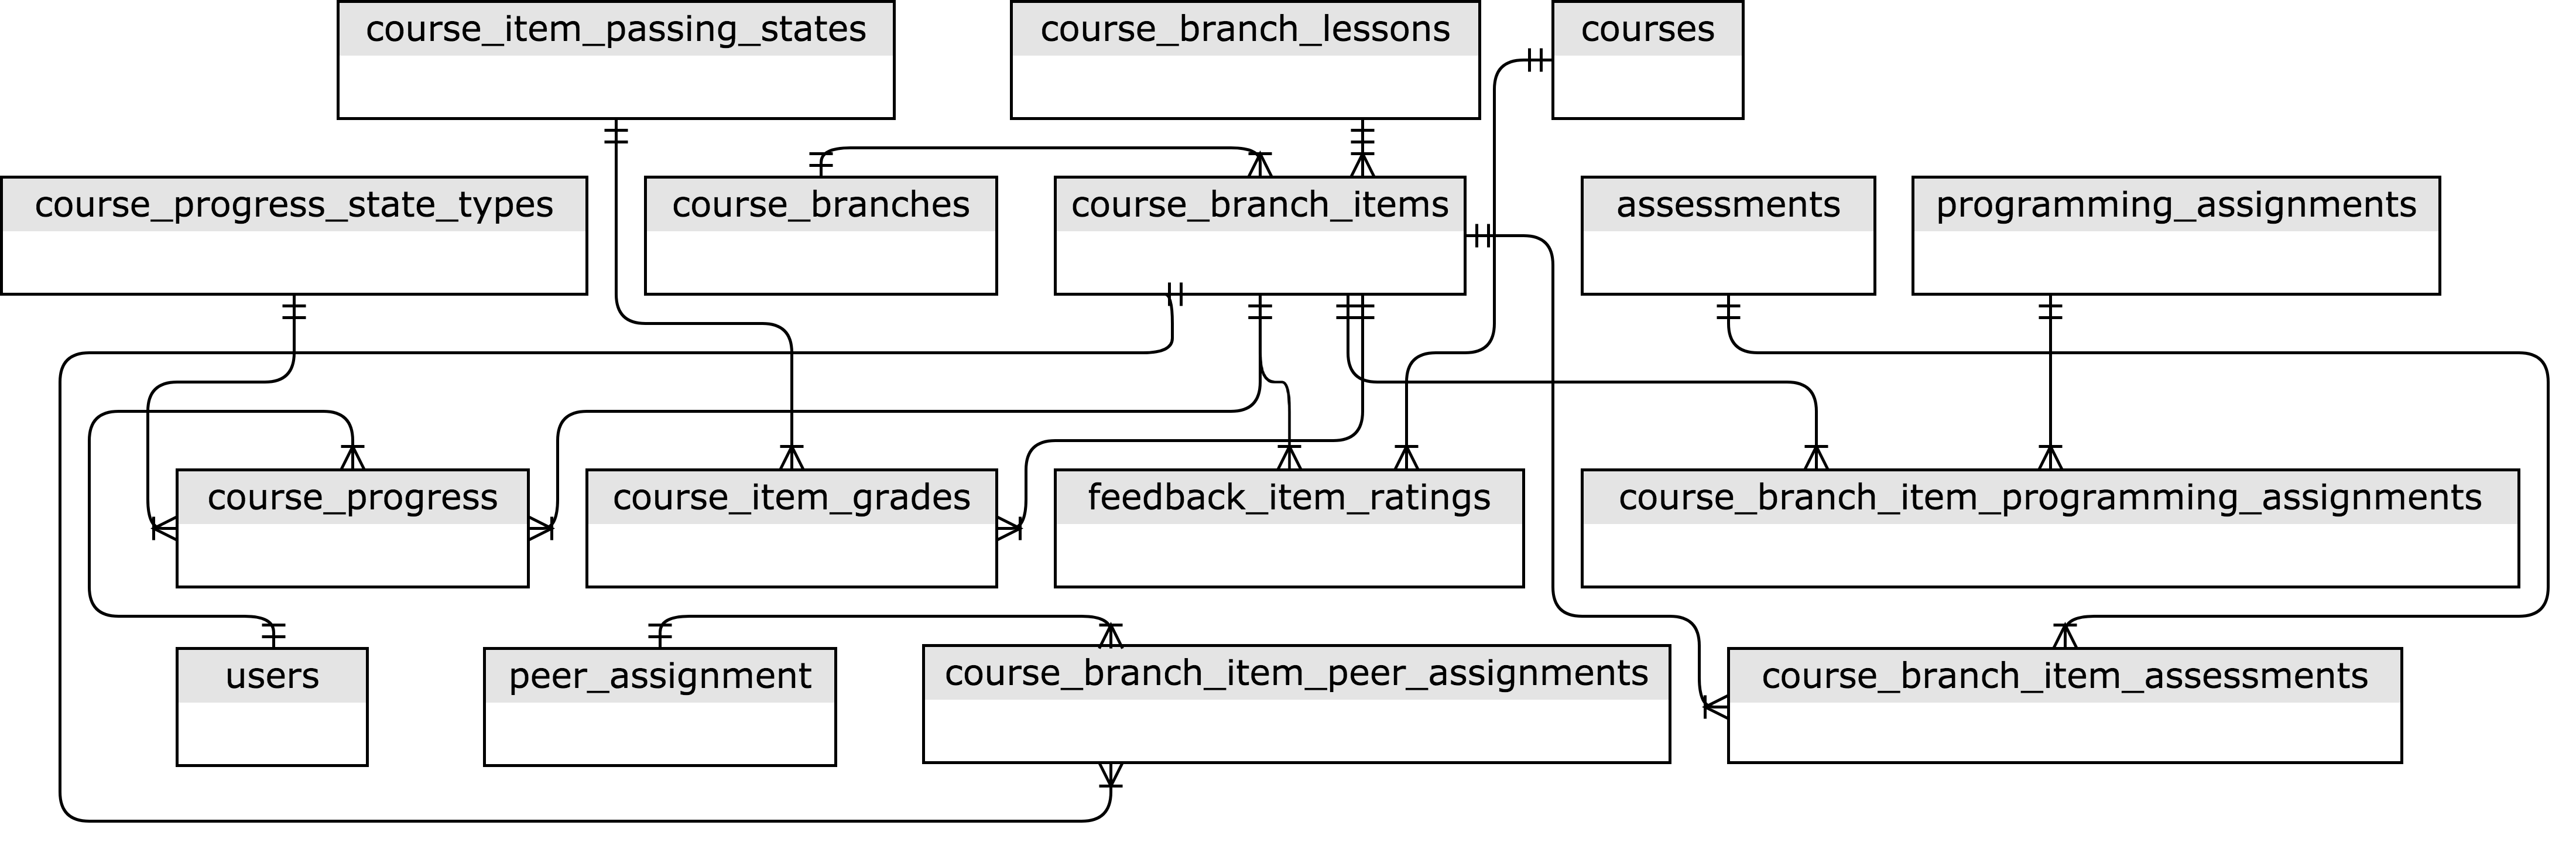
\includegraphics[scale=0.5]{datatables}
    \caption{The major relationships between tables groups, with minor connections omitted (Source: Coursera)}
    \label{figure:datatables}
\end{figure}

While Coursera provides tools for creating Postgres databases in a
docker
container\footnote{The tools is called `courseraresearchexports` and can be found here: https://github.com/coursera/courseraresearchexports},
as we mentioned earlier, importing data for analysis remains to be a
challenge for researchers with limited experience with relational
databases. Moreover, such tools are usually not platform
independent.\footnote{In an initial version of `crsra` based on Postgresql we had the problem of some team members not being able to set up the database properly on their PCs.}

\subsection{Importing Data Using
crsra}\label{importing-data-using-crsra}

write about data from coursera's gitbook size of data examples of
hopkins courses provide a list of tables that connect different
students.

Talk about the advantage of not having relational databses

data can only be downloaded by ``a single instructor to refine his/her
own course or a research team at your institution (admins and data
coordinators), to support broader online pedagogy initiatives''

Research data exports are sets of CSV files, designed for use in
relational database systems. You can choose from a list of data types to
download. Data coordinators can also use a single hashed user ID in all
data domains. Learn more about data types and hashed user IDs.

To download export files: Access self-service exports Scroll to the
``Research Data'' section and choose the types of data you want to
download (select all that apply) Type a ``Purpose for requesting
exports'' (e.g.~how you plan to use the data, what research questions
you're asking, who will work with the data, who you'll share it with,
etc.) Data coordinators: To use a single hashed user ID in all data
domains, check the ``Learner Identity Exposure'' box Click Export
Completed exports are displayed in the ``Data Export History'' section.
Click Download to save the files.

\subsection{crsra Package}\label{crsra-package}

talk about the package

\subsection{Analysis of student behavior on
Coursera}\label{analysis-of-student-behavior-on-coursera}

provide the analaysis here

\subsection{Discussion}\label{discussion}

\bibliography{RJreferences}

\address{%
Aboozar Hadavand\\
Bloomberg School of Public Health, Johns Hopkins University\\
615 N. Wolfe Street\\ Baltimore, MD 21205, USA\\
}
\href{mailto:hadavand@jhu.edu}{\nolinkurl{hadavand@jhu.edu}}

\address{%
Jeffrey Leek\\
Bloomberg School of Public Health, Johns Hopkins University\\
615 N. Wolfe Street\\ Baltimore, MD 21205, USA\\
}
\href{mailto:jtleek@jhu.edu}{\nolinkurl{jtleek@jhu.edu}}

